% Paper sections as of 8 Nov 2026 (copied from the NAMRC 55 manuscript).
% Requires booktabs, graphicx and the bibliography entries bednarik2018tds, ronneberger2015unet, shi2015convlstm.
\section{Results}

\subsection{Model Training}
All servo runs completed. The 30-epoch reference model reached its lowest validation objective, 10.13~mm, at epoch 26. Among the 100-epoch models trained with standard masks, the model trained from scratch selected epoch 85 (8.65~mm) and the cloth-pretrained model epoch 49 (9.35~mm). The mixed-mask models selected epochs 98 (10.00~mm, from scratch) and 72 (10.75~mm, cloth-pretrained); the model trained from scratch therefore became the primary model. Mixed-mask objectives were computed with mixed validation masks and are not comparable with those of the standard-mask models. The primary model's best epoch was close to the 100-epoch limit, so longer training might reduce its error further. Cloth pretraining stopped early at epoch 37 and retained epoch 29. Each 100-epoch servo run took about 0.5~h on the RTX 5090. Of the 1,168 candidate training windows, 40 were excluded for frame-interval violations; three of the 1,743 candidate test windows were excluded for the same reason, and no window was excluded for insufficient coverage.

\subsection{Synthetic Occlusion on Held-Out Motions}
Table~\ref{tab:synthetic} summarizes the 1,740 test windows from the stop--start and biased-oscillation recordings under both mask types, and Fig.~\ref{fig:synthetic_lead} shows the hidden-cell error at each forecast step.

\begin{table*}[t]
\centering
\caption{Held-out synthetic-occlusion results (1,740 test windows from the stop--start and biased-oscillation recordings; identical windows and masks for every model). Values are hidden-cell MAE in millimeters of camera-axis depth, current / 200~ms.}
\label{tab:synthetic}
\vspace{4pt}
\small
\begin{tabular}{lccc}
\toprule
 & \multicolumn{2}{c}{Standard masks (20\% of grid, moving)} & Large masks (70--90\%, stationary) \\
\cmidrule(lr){2-3}\cmidrule(lr){4-4}
Model & Observed earlier in window\textsuperscript{a} & All hidden cells & All hidden cells \\
\midrule
Mixed masks, 100 epochs (primary)           & 2.48 / 3.20 & 2.56 / 2.79 & \phantom{0}3.28 / \phantom{0}3.29 \\
Mixed masks, 100 epochs, cloth-pretrained   & 2.49 / 3.50 & 2.73 / 3.10 & \phantom{0}3.61 / \phantom{0}3.65 \\
Standard masks, 100 epochs                  & 2.47 / 3.17 & 2.56 / 2.76 & 36.31 / 36.57 \\
Standard masks, 100 epochs, cloth-pretrained & 2.48 / 3.51 & 2.74 / 3.12 & 28.08 / 19.68 \\
Standard masks, 30 epochs (reference)       & 2.60 / 3.49 & 2.68 / 2.98 & 20.61 / 20.41 \\
\midrule
Last observation                            & 3.58 / 4.40 & --\textsuperscript{b} & --\textsuperscript{b} \\
\bottomrule
\end{tabular}

\smallskip
\parbox{\linewidth}{\footnotesize
\textsuperscript{a}Hidden cells the last-observation baseline can estimate (59,579 of 272,219 current targets); model and baseline are scored on the same cells.
\textsuperscript{b}The baseline cannot estimate cells never observed in the input window (78\% of hidden targets under standard masks, all under large masks).}
\end{table*}

\begin{figure*}[t]
\centering
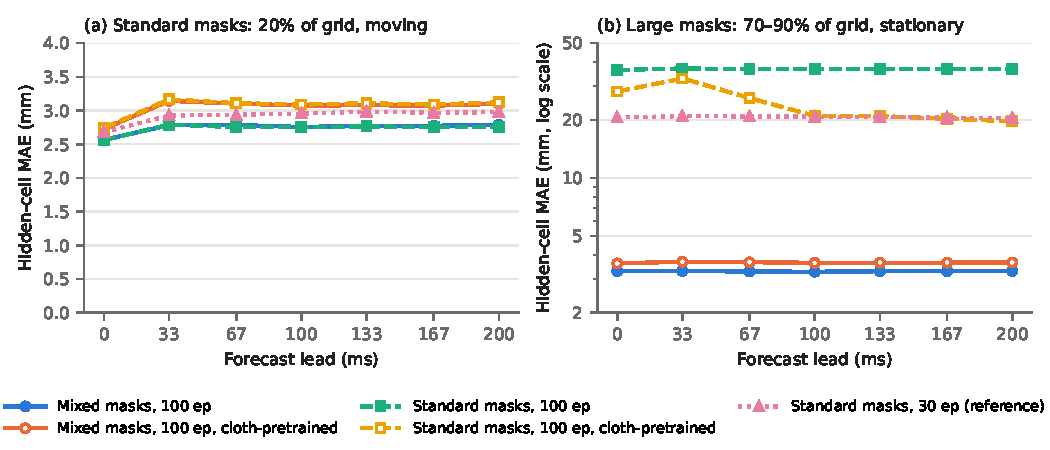
\includegraphics[width=\textwidth]{figures/occlusion_mae_vs_lead.pdf}
\caption{Hidden-cell mean absolute error against forecast lead on the held-out motions, for all hidden cells with valid targets. (a) Standard masks covering 20\% of the grid and moving. (b) Large stationary masks covering 70--90\% of the grid (log scale). Solid lines: models trained with mixed masks; dashed and dotted lines: models trained with standard masks only; open markers: cloth-pretrained models.}
\label{fig:synthetic_lead}
\end{figure*}

With standard masks, training for 100 epochs reduced hidden-cell errors relative to the 30-epoch reference, and mixed-mask training preserved this accuracy. On hidden cells that the last-observation baseline could support, the primary model's current and 200~ms errors were 2.48 and 3.20~mm, compared with 2.47 and 3.17~mm for the corresponding standard-mask model, 2.60 and 3.49~mm for the reference, and 3.58 and 4.40~mm for the baseline. Over all hidden cells with valid targets, 78\% of which had not been observed anywhere in the input window, its errors were 2.56 and 2.79~mm. Cloth pretraining did not improve these results: both pretrained models had 200~ms errors of 3.50--3.51~mm on supported hidden cells.

The 100-epoch models reproduced visible measurements more closely than the reference, with current visible-cell errors of 0.35--0.67~mm compared with 1.71~mm. Most forecast error appeared at the first step: for the primary model, the visible-cell error was 2.78~mm at 33~ms and 2.79~mm at 200~ms, and the baseline's was 3.72 and 3.75~mm. The baseline's one-frame error indicates substantial frame-to-frame variation in the measured maps, so much of the error at every lead likely reflects measurement variation rather than surface displacement over the horizon. The windows overlap in time and are not independent trials.

With large stationary masks, every model trained with standard masks failed. Their current hidden-cell errors were 20.61~mm for the reference, 36.31~mm for the 100-epoch model and 28.08~mm for its cloth-pretrained counterpart, compared with 2.56--2.74~mm for the same models under standard masks. Mixed-mask training removed most of this failure: the primary model's current and 200~ms errors were 3.28 and 3.29~mm, and those of the cloth-pretrained mixed-mask model were 3.61 and 3.65~mm. On visible cells at 200~ms, the primary model's error was 3.35~mm, compared with 4.47~mm for the last-observation baseline.

\subsection{Real Print-Head Occlusion}
The stationary head mask left 15.4--17.9\% of grid cells observed in the scored windows of the five reserved patterns, compared with 54\% in the standard-mask test windows, so the real-head condition resembled the large-mask test more closely. In total, 3,836 windows were scored at the current lead and 3,699 at 200~ms (Table~\ref{tab:realhead}).

Before any prediction, the two recordings of each pattern differed by 5.45~mm in camera depth on cells visible in both within the scored windows (mean offset $+4.95$~mm, blocked minus reference), equivalent to 2.92~mm vertically in the printer frame (offset $-2.68$~mm). Differences between the models' estimates and the reference recordings must be read against this run-to-run disagreement.

\begin{table*}[t]
\centering
\caption{Real print-head recordings compared with separate, unregistered repeat recordings, within the masked region. Values are mean absolute differences in millimeters, current / 200~ms, with the current mean offset (prediction minus reference). They are not ground-truth errors.}
\label{tab:realhead}
\vspace{4pt}
\small
\begin{tabular}{lcccc}
\toprule
 & \multicolumn{2}{c}{Camera-axis depth} & \multicolumn{2}{c}{Printer height\textsuperscript{a}} \\
\cmidrule(lr){2-3}\cmidrule(lr){4-5}
Model & Difference & Offset & Difference & Offset \\
\midrule
Mixed masks, 100 epochs (primary)            & \phantom{0}8.82 / \phantom{0}7.92 & \phantom{0}$+7.71$ & \phantom{0}4.02 / \phantom{0}3.61 & \phantom{0}$-3.54$ \\
Mixed masks, 100 epochs, cloth-pretrained    & \phantom{0}6.61 / \phantom{0}5.07 & \phantom{0}$+5.70$ & \phantom{0}2.97 / \phantom{0}2.27 & \phantom{0}$-2.61$ \\
Standard masks, 100 epochs                   & 33.80 / 36.07 & $-33.73$ & 15.85 / 16.84 & $+15.81$ \\
Standard masks, 100 epochs, cloth-pretrained & 14.50 / 11.21 & $+11.83$ & \phantom{0}6.59 / \phantom{0}5.22 & \phantom{0}$-5.40$ \\
Standard masks, 30 epochs (reference)        & \phantom{0}5.79 / \phantom{0}5.21 & \phantom{0}$+0.45$ & \phantom{0}2.64 / \phantom{0}2.35 & \phantom{0}$-0.22$ \\
\midrule
Repeat recordings, visible cells\textsuperscript{b} & \phantom{0}5.45 / \phantom{0}5.44 & \phantom{0}$+4.95$ & \phantom{0}2.92 / \phantom{0}2.91 & \phantom{0}$-2.68$ \\
\bottomrule
\end{tabular}

\smallskip
\parbox{\linewidth}{\footnotesize
\textsuperscript{a}Printer Z of the prediction minus that of the reference surface at the same printer XY, using the provisional registration; positive means too high.
\textsuperscript{b}Last observation of the blocked recording against the repeat recording on cells visible in both, before prediction; the run-to-run disagreement. Scored windows: 3,836 current, 3,699 at 200~ms.}
\end{table*}

Mixed-mask training reduced the real-head differences of the 100-epoch models. In camera depth, the current hidden-region difference fell from 33.80 to 8.82~mm for models trained from scratch and from 14.50 to 6.61~mm for cloth-pretrained models; in printer height, it fell from 15.85 to 4.02~mm and from 6.59 to 2.97~mm. The 100-epoch standard-mask model placed the hidden surface about 34~mm too near the camera, nearly 16~mm too high in the printer frame. The 30-epoch reference differed by 5.79~mm in camera depth and 2.64~mm in printer height. The reference and the cloth-pretrained mixed-mask model were therefore at the level of the run-to-run disagreement in printer height (2.92~mm), and this comparison cannot rank them; the large-mask test, which has true labels, separates them (20.61 versus 3.61~mm). For both mixed-mask models, the seeded random walk gave the smallest current difference of the five patterns (5.13 and 4.95~mm in camera depth), whereas it had given the largest for the reference (8.56~mm).

Taken together, the large-mask test and the real print-head comparison agree that models trained only with small moving masks do not generalize to head-scale occlusion, and that mixed-mask training addresses this without loss under small masks. The real-head comparison remains limited by an unregistered repeat reference, a provisional printer registration, and a single training run per configuration; it does not establish hidden-surface accuracy. That requires a synchronized independent measurement of the surface behind the head, or a validated registration between runs, together with a measured per-frame head mask.


